% bei Standalone in documentclass noch:
% \RequirePackage{luatex85}

\documentclass[captions=tableheading, titlepage= firstiscover, parskip = half , bibliography=totoc]{scrartcl}
%paper = a5 für andere optinen
% titlepage= firstiscover
% bibliography=totoc für bibdateien
% parskip=half  Veränderung um Absätze zu verbessern

\usepackage{scrhack} % nach \documentclass
\usepackage[aux]{rerunfilecheck}
\usepackage{polyglossia}
\usepackage[style=numeric, backend=biber]{biblatex} % mit [style = alphabetic oder numeric] nach polyglossia
\addbibresource{lit.bib}
\setmainlanguage{german}

\usepackage[autostyle]{csquotes}
\usepackage{amsmath} % unverzichtbare Mathe-Befehle
\usepackage{amssymb} % viele Mathe-Symbole
\usepackage{mathtools} % Erweiterungen für amsmath
\usepackage{fontspec} % nach amssymb
% muss ins document: \usefonttheme{professionalfonts} % für Beamer Präsentationen
\usepackage{longtable}

\usepackage[
math-style=ISO,    % \
bold-style=ISO,    % |
sans-style=italic, % | ISO-Standard folgen
nabla=upright,     % |
partial=upright,   % /
]{unicode-math} % "Does exactly what it says on the tin."
\setmathfont{Latin Modern Math}
% \setmathfont{Tex Gyre Pagella Math} % alternativ

\usepackage[
% die folgenden 3 nur einschalten bei documenten
locale=DE,
separate-uncertainty=true, % Immer Fehler mit ±
per-mode=symbol-or-fraction, % m/s im Text, sonst \frac
]{siunitx}

% alternativ:
% per-mode=reciprocal, % m s^{-1}
% output-decimal-marker=., % . statt , für Dezimalzahlen

\usepackage[
version=4,
math-greek=default,
text-greek=default,
]{mhchem}

\usepackage[section, below]{placeins}
\usepackage{caption} % Captions schöner machen
\usepackage{graphicx}
\usepackage{grffile}
\usepackage{subcaption}

% \usepackage{showframe} Wenn man die Ramen sehen will

\usepackage{float}
\floatplacement{figure}{htbp}
\floatplacement{table}{htbp}

\usepackage{mhchem} %chemische Symbole Beispiel: \ce{^{227}_{90}Th+}


\usepackage{booktabs}

 \usepackage{microtype}
 \usepackage{xfrac}

 \usepackage{expl3}
 \usepackage{xparse}

 % \ExplSyntaxOn
 % \NewDocumentComman \I {}  %Befehl\I definieren, keine Argumente
 % {
 %    \symup{i}              %Ergebnis von \I
 % }
 % \ExplSyntaxOff

 \usepackage{pdflscape}
 \usepackage{mleftright}

 % Mit dem mathtools-Befehl \DeclarePairedDelimiter können Befehle erzeugen werden,
 % die Symbole um Ausdrücke setzen.
 % \DeclarePairedDelimiter{\abs}{\lvert}{\rvert}
 % \DeclarePairedDelimiter{\norm}{\lVert}{\rVert}
 % in Mathe:
 %\abs{x} \abs*{\frac{1}{x}}
 %\norm{\symbf{y}}

 % Für Physik IV und Quantenmechanik
 \DeclarePairedDelimiter{\bra}{\langle}{\rvert}
 \DeclarePairedDelimiter{\ket}{\lvert}{\rangle}
 % <name> <#arguments> <left> <right> <body>
 \DeclarePairedDelimiterX{\braket}[2]{\langle}{\rangle}{
 #1 \delimsize| #2
 }

\setlength{\delimitershortfall}{-1sp}

 \usepackage{tikz}
 \usepackage{tikz-feynman}

 \usepackage{csvsimple}
 % Tabellen mit \csvautobooktabular{"file"}
 % muss in table umgebung gesetzt werden


% \multicolumn{#Spalten}{Ausrichtung}{Inhalt}

\usepackage{hyperref}
\usepackage{bookmark}
\usepackage[shortcuts]{extdash} %nach hyperref, bookmark

\newcommand{\ua}[1]{_\symup{#1}}
\newcommand{\su}[1]{\symup{#1}}


\begin{document}

\section{Einleitung und Idee}

Als es darum ging ein Thema für unseren Zusatzversuch rauszusuchen, haben wir uns
eigentlich sofort für die Wirbelstrombremse entschieden. Einerseits gehört sie zu
dem Bereich des Magnetismus und wurde in der Physik II schon ausführlich behandelt,
so dass wir mit dem Thema schon vertraut waren. Andererseits ist es ein Prinzip,
dass auch im Alltag sehr viel Anwendung findet. Somit ist es ein eigentlich sehr
allgemeines Thema, dass zu dem auch sehr viele Möglichkeiten für ein Experiment
bietet.

\section{Aufbau}

Wir hatten für unseren Versuch eigentlich einen ziemlich klaren Aufbau im Kopf,
den wir bei der tatsächlichen Versuchsdurchführung jedoch etwas abändern mussten.
Theoretisch wollten wir uns bei unserem Versuch stark an dem Waltenhofeschen Pendel
orientieren. Bis auf ein paar kleine Umänderungen kam unser Aufbau auch ziemlich
nahe an dieses Vorbild heran. Grundsätzlich bestand der Aufbau dabei aus nicht
allzu vielen Bestandteilen:

\begin{itemize}
  \item 2 Magnetspulen
  \item 1 großer U-Eisenkern, 2 kleine Eisenkerne
  \item 1 Stativ mit Pendel
  \item 2 große Hebewagen, 1 kleiner Hebewagen
  \item 1 Stromgenerator
  \item 3 Aluminiumplatten
  \item mehrere Stromkabel
\end{itemize}



\section{Anwendungsbeispiele}

Ein Beispiel dafür ist der Einsatz bei Schienenfahrzeugen. Hier wird in zwei
Kategorien bzw. Techniken unterschieden, die lineare und die rotierende Wirbelstrombremse.
Bei der linearen Wirbelstrombremse wird dabei ein zu den Schienen paralleles
Magnetfeld mithilfe eine Reihe von Magneten, die über einen Integralträger und
Tragärme am Radsatzlager befestigt sind. Diese Magneten werden bei Aktivierung
auf ca. 7 mm Entfernung über die Schienen gesenkt, so dass ein längs zu der Schiene
verlaufendes Magnetfeld erzeugt wird.

\begin{figure}
  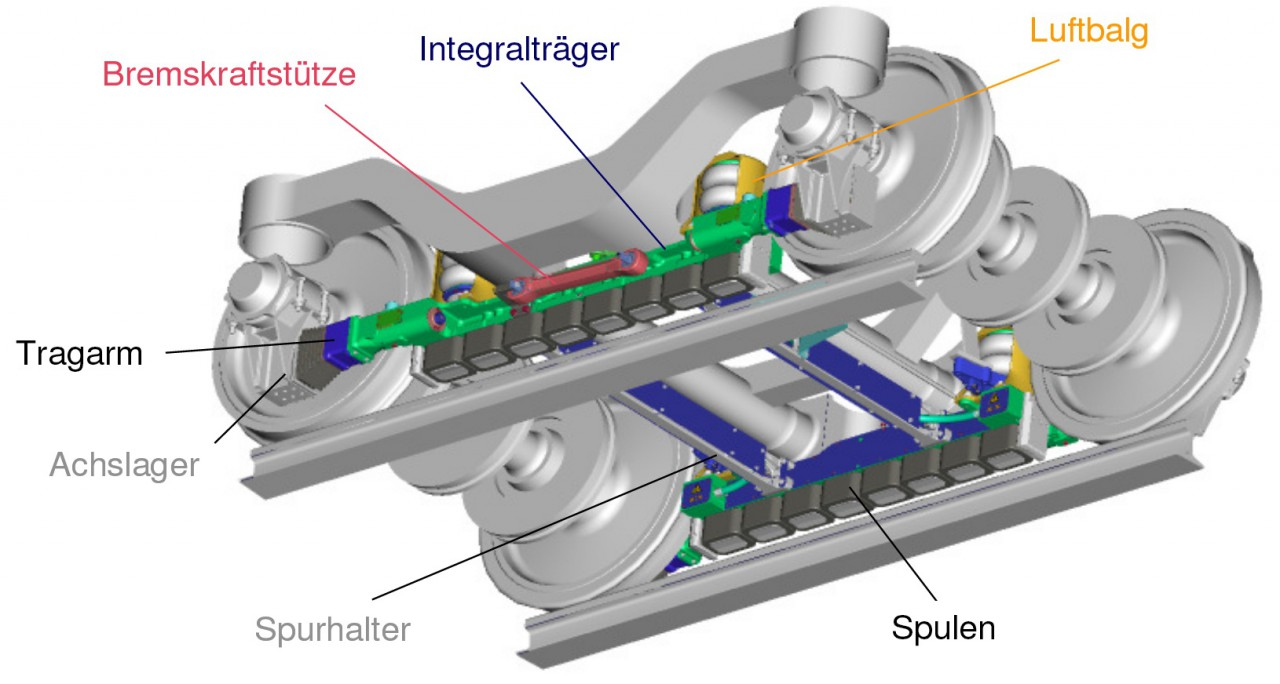
\includegraphics[width=\textwidth]{Wirbelstrombremse_Aufbau.jpg}
  \caption{Aufbau einer linearen Wirbelstrombremse}
  \label{fig:linWAufbau}
\end{figure}

Diese Variante
wird allerdings nur bei sehr hohen Geschwindigkeiten sowie auf extra eingerichteten
Schienen verwendet.
Bei der rotierenden Wirbelstrombremse hingegen wird die Schiene als Elektromagnet
verwendet um Wirbelströme in den Rädern des Zuges zu erzeugen. Diese Variante wird
zurzeit allerdings nur bei Versuchsfahrzeugen eingesetzt bzw. getestet.


\end{document}
